% SPF Report:
\documentclass[english]{SFOEYearlyReportEnglish_2018}


\usepackage{subfigure}

\usepackage{ragged2e}
\usepackage{setspace}
\usepackage{scrextend}
\usepackage{xspace}
\usepackage{siunitx}

\sisetup{detect-all=true}
\usepackage[printonlyused,nohyperlinks]{acronym}

%\sisetup{
%detect-family=true,
%detect-weight=true,
%detect-mode=true,
%detect-display-math = false
%}

\def\italictitle#1{\par\vspace{10pt}\centerline{\it #1}\par\vspace{10pt}}
\DeclareSIUnit \spf{~$SPF_{SHP+}$}


\reportDate{\textbf{Annual report 2020} } % or write the date manually 
\reportName{Slurry-Store}
\reportSubName{Experimental and numerical investigations of ice slurry storages.}


\newcommand{\OneFigLocal}[3]{
\begin{figure}[!ht]
\begin{center}
 \includegraphics[width=1 \textwidth]{#1} 
 \vspace{-0.75cm}
\caption{#2}
 \label{#3}
 \end{center}
  \vspace{-1cm}
 \end{figure}
 }
 
% \setlength{\textfloatsep}{10pt plus 1.0pt minus 2.0pt} no effect
\setlength\belowcaptionskip{-10pt}


\begin{document} 

%%% COMMANDS
%%
%% \acresetall	flushes the ’memory’ of the macro \ac (ie all "used" marks flushed)
%%
%% \ac{label}	singular (first time Full Name + (ACRO) and mark as used)
%% \acp{label}	plural (as \ac but makes short and/or long forms into plurals)
%%
%% \acs{lable}	short (ACRO)
%% \acf{lable}	“full acronym” (Full Name + (ACRO))
%% \acl{lable}	long (_without_ ACRO)
%%
%% \acsp{label}	short plural (ACROs)
%% \acfp{label}	“full acronym” plural (Full Names + (ACROs))
%% \aclp{label}	long plural (_without_ ACRO)
%%
%% \acrodef{label}[acronym]{written out form}	definition
%%		for example \acrodef{etacar}[$\eta$ Car]{Eta Carinae},
%%		with the restriction that the label should be simple ASCII


%% PACKAGE & OPTIONS
%% acronym package must be loaded (in the preamble):
%%    \usepackage[option1,option2,etc.]{acronym}
%% OPTIONS:
%%    footnote		The option footnote makes the full name appear as a
%%			footnote.
%%    nohyperlinks	If hyperref is loaded, all acronyms will link to their
%%			glossary entry. With the option nohyperlinks these
%%			linkscan be suppressed.
%%    printonlyused	Only list used acronyms
%%    withpage		In printonlyused-mode show the page number where
%%			each acronym was first used.
%%    smaller		Make the acronym appear smaller.
%%    dua			The option dua stands for “don’t use acronyms”. It
%%			leads to a redefinition of \ac and \acp, making the
%%			full name appear all the time and suppressing all
%%			acronyms but the explicity requested by \acf or \acfp.
%%    nolist		The option nolist stands for “don’t write the list of
%%			acronyms”.


%% INCLUSION
%%

\begin{acronym}[OMNeTXX] %width of the longest acronym should be matched here

\section*{List of Acronyms}
\label{sec:acronyms}

  %\acro{h2o}[$\mathrm{H_2O}$]{water}
  \acro{ASHP}{Air Source Heat Pump}
  \acro{CA}{Static contact angle}
  \acro{CA_{adv}}{Advancing contact angle}
  \acro{CA_{rec}}{Receding contact angle}
  \acro{CAH}{Contact angle hysteresis}
  \acro{COP}{Coefficient Of Performance}
  \acro{CM}{Capillary mats}
  \acro{d1}{Coating based on hybrid organic/inorganic sol-gel}
  \acro{d2}{Coating based on silicon rubber}
  \acro{DHW}{Domestic Hot Water}

  \acro{FP}{Flat plate}
  
  \acro{GWP}{Global Warming Potential}
  \acro{GSHP}{Ground Source Heat Pump}
  \acro{ASHP}{Ground Source Heat Pump}
 \acro{HTF} {Heat Transfer Fluid}
 \acro{HX} {Heat Exchanger}

  \acro{ice-on-hx}{Ice on Heat Exchanger}
  \acro{MFH} {Multi Family Home}
  \acro{m2}{Coating based on fluorochemical modified urethanes}
  \acro{PP}{PolyPropylene}
  \acro{PV}{Photovoltaics}
  \acro{Ra}{Surface roughness}

  \acro{SAHP}{Solar Assisted Heat Pump}
  \acro{SFH} {Single Family Home}
  \acro{MFH} {Multy Family Home}

  \acro{SPF}{Seasonal Performance Factor}
  \acro{SS}{Stainless Steel}

  \acro{SSHP}{Solar Source Heat Pump}
  \acro{IRF}{Ice reduction factor}
  
  \acro{CNT}{Classical nucleation theory}
  
  %\acro{ice-on-coil}{Ice built on the surface of coil based heat exchangers}
  %\acro{ice-on-plates}{Ice built on the surface of plate base heat exchangers}

%\section*{List of Symbols}
%\label{sec:symbols}
%\acro{$Q_D$}{Total heating energy demand}
%%\si{Q_{SH,tFl}}
%\acro{QShTfl}[$Q_{SH,tFl}$]{Heat flow of Space Heating loop as function of the flow Temperature}
%\acro{QShTrt}[$Q_{SH,tRt}$]{Heat flow of Space Heating loop as function of the return Temperature}
% \acro{QD}[$Q_{D}$]{Total Heat demand}
% \acro{QSH}[$Q_{sh}$]{Space heat demand}
% \acro{QDHW}[$Q_{dhw}$]{Domestic hot water heat demand} 
% \acro{Tfl}[$T_{fl}$]{Flow temperature of the heating distribution system} 
% \acro{Trt}[$T_{rt}$]{Return temperature of the heating distribution system} 
%\acro{Qcond}[$Q_{cond}$]{Heat provided by the heat pump condenser} 
%\acro{Qevap}[$Q_{evap}$]{Heat needed by the heat pump evaporator}
%\acro{Qice}[$Q_{ice}$]{Latent heat extracted from the ice storage}
%\acro{QColToTes}[$Q_{col\rightarrow tes}$]{Heat provided from solar collectors to the thermal storage tank}
%\acro{QcolToHp}[$Q_{col\rightarrow hp}$]{Heat provided from solar collectors to the heat pump evaporator}
%\acro{QcolToIce}[$Q_{col\rightarrow ice}$]{Heat provided from solar collectors to the ice storage}


  
\end{acronym}
\newpage


\section{Motivation}

Solar-ice systems are becoming more and more popular in Switzerland. However, state-of-the-art solar-ice systems have some disadvantages such as a usually higher cost compared to Ground Source Heat Pumps GSHP if the same performance is desired. Therefore, research is still needed to bring robust solar-ice systems to the market with comparable cost and higher efficiency with respect to ground-source heat pump solutions. 
The solar ice-slurry system is a particular case of solar-ice systems. The main difference between them is that in the ice slurry concept the ice storage contains no heat exchangers, which reduces the system installation cost by 10~\%. Moreover, the heat exchanger (supercooler) is always free of ice and thus has a higher efficiency compared to ice-on-coil (15~\% higher at 50~\% ice fraction) and there is no need to de-ice them compared to the thermal de-icing concept. A feasibility study carried out in the project Slurry HP undertaken by SPF \cite{SlurryHp_2017} has shown that solar-ice systems based on the ice slurry heat pump using the supercooling approach have a high potential for cost reduction, while having a high energetic efficiency, especially for ice storage volumes of at least \SI{1}{m^3} per MWh of yearly heating demand, which corresponds well to ice storage volumes used today for multi-family buildings. Moreover, an ice slurry storage would allow to use existing rooms of the building efficiently since any shape and room size could store slurries if properly distributed.
Within Slurry-HP, the system energetic efficiencies, investment and heat generation costs were compared to the best performing simulated solar-ice configuration as well as to current GSHP systems. An example of the simulated system efficiencies and estimated heat generation cost for a single family house (SFH) in Zurich is shown in Fig.~\ref{fig:solar-ice} with the corresponding reference cost for a GSHP (cost based on different offers from companies). From Fig~\ref{fig:solar-ice} it can be observed that a solar ice-slurry system with \SI{1.5}{m^2} of collector area and \SI{1}{m^3} of ice storage volume per MWh of heat demand has an efficiency (\si{\spf}) of 4.8 with lower heat generation cost compared to GSHP systems.
%\SIrange{10}{20}{m^2}, \SIlist{10;20;30}{m^2}

\begin{figure}[!htbp]
    \centering
    %trim={<left> <lower> <right> <upper>}
    %\includegraphics[trim={0 0 0 0},clip,width=0.8\textwidth]{figures/}
    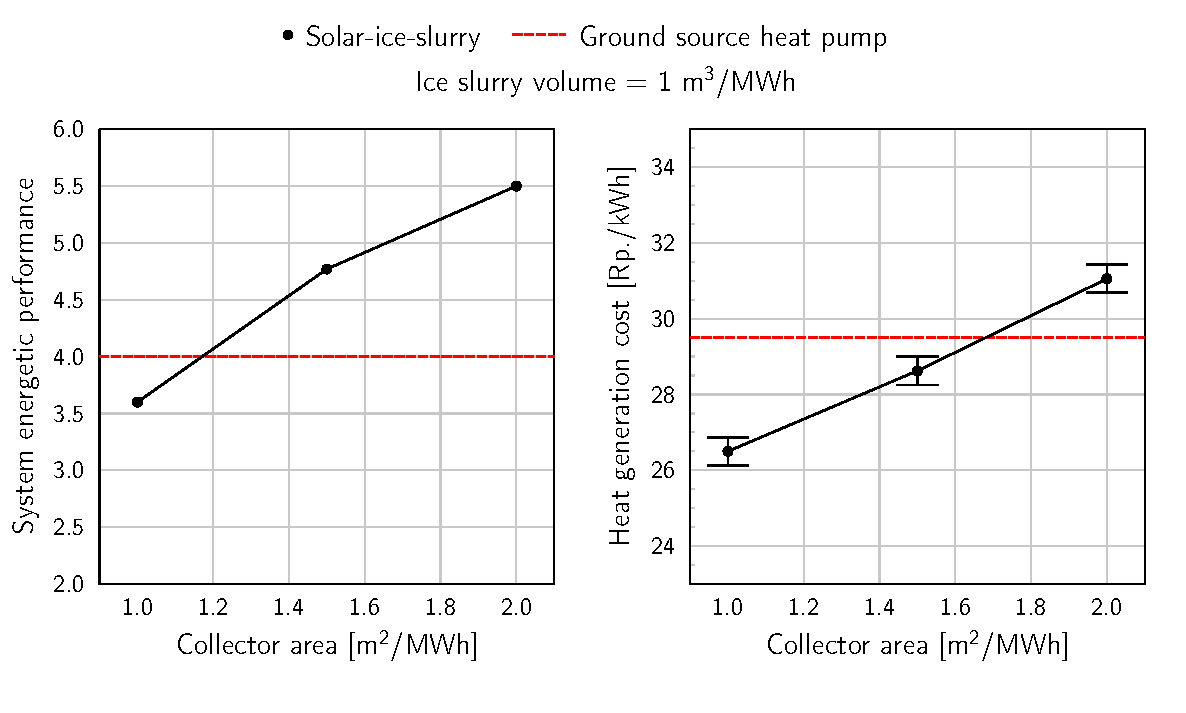
\includegraphics[trim={0 0 0 0},clip,width=0.8\textwidth]{figures/cost-Slurry-direct-large-errorBar.pdf}
    \caption{Comparison between a solar-ice slurry solution based on a supercooling and the GSHP system in terms of \si{\spf} and heat generation cost.}
   \label{fig:solar-ice}
\end{figure}


\section{Project objectives}

The overall goal of the Slurry-Store project will be to experimentally investigate ice storages able to store and melt slurries with (solar) heat without using any mixing device.
The specific objectives of the project will be:
\begin{itemize}
    \item Design, built and test an ice slurry storage design able to achieve 50~\% ice slurry fraction
    \item Develop and test an ice releaser for stable continuous operation of 6 hours
    \item Design, built and test two concepts for loading (icing)
    \item Design, built and test two concepts for unloading (melting)
    \item Develop a mathematical formulation for the ice slurry storage, implement it and validated within TRNSYS.
\end{itemize}

\section{Status and work carried out}

\subsection{Experimental set-up}

\begin{figure}[!htbp]
    \centering
    %trim={<left> <lower> <right> <upper>}
    %\includegraphics[trim={0 0 0 0},clip,width=0.8\textwidth]{figures/}
    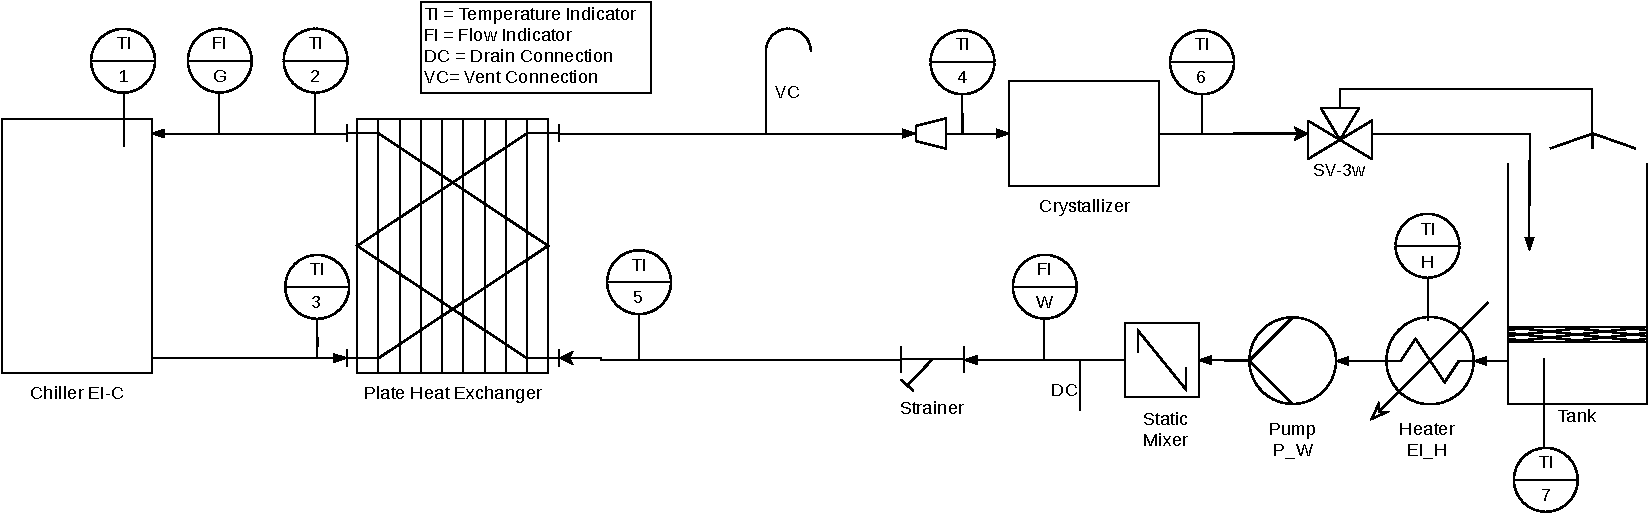
\includegraphics[trim={0 0 0 0},clip,width=\textwidth]{figures/SetUp_v01.pdf}
    \caption{Piping \& Instrumentation Diagram of the planned set up.}
   \label{fig:setup}
\end{figure}

\noindent
 The goal of the described installation is to continuously produce an ice  slurry with an ice content of roughly 2~\% at the tank inlet, and up to 50\% of ice in the tank itself. Its design is based on the setup of a previous project, in which the supercooling capability of a coated double tube heat exchanger was tested. The setup consists of two separate piping loops: A water loop with demineralized water and a glycol-water loop with 30\% glycol as refrigerant. The two loops are connected via a plate heat exchanger that acts as supercooler of the water. Both loops are designed from 1" plastic pipes and a flow of \SIrange{200}{2000}{l/h}.


In the \textbf{Water-loop}. starting at the water/ice tank, the water is heated up to \SI{0.5}{\celsius} to ensure that no leftover ice particles from the tank can be found within the stream. The fluid is then pumped through the water loop using a radial pump "P\_W" (Grundfos CME). After passing a static mixer that ensures homogeneousity of the temperature in the flow, the mass of the flow is measured using a Coriolis mass flow meter (DN15, E+H, Promass E300, "FI-W"). It then passes a filter with \SI{0.5}{mm} mesh size (+GF+ Strainer Type 305) to remove possible solid particles before it reaches the supercooler. In this welded plate type heat exchanger (AlfaLaval), the water is cooled down to temperatures between \SIrange{0}{-2}{\celsius}, where coated supercooler walls are expected to prevent formation of ice. Directly after the supercooler, the supercooled water is crystallized in the custom made crystallizing pipe section. Parts of the water are cooled electrically using peltier modules to promote crystallization. This step is crucial to prevent formation of ice in unwanted places, where the ice could block the pipe. Since ice is reported to propagate upstream along the pipe walls  \citep{mito_new_2002}, heat tracing is used to locally increase the pipe walls above freezing temperature. At the location of the crystallizer, the pipe diameter is increased to \si{3}{"} to reduce the flow velocity to increase the time for ice to grow. The ice slurry then leaves the crystallizer and is passed on to the tank. Between the crystallizer and the tank, a tree way valve is placed. With this valve, a de-icing programm can be run, where warmed water is sprayed from the top onto floating ice inside the tank.


The \textbf{glycole loop} acts as the refrigerant, and is cooled using the heat pump IN 1030 T. Its flow is generated using a pump within the heat pump and controlled by a MID "FI-G". The temperature is controlled using PT-100 within the  heat pump and before and after the heat exchanger.

Temperatures are measured using seven 4-wire PT100 temperature indicators. TI-2 to -5 are used to generate an energy balance calculation across the supercooling plate heat exchanger. TI-5 is also used to control the heat generated by the heater EI-H. TI-H acts as safety instrument to prevent the heater from overheating if it sould run dry. The temperature difference between TI-4 and -5 is used to check proper ice generation. A negative temperature in -4 and a temperature of \SI{0}{\celsius} indicates complete release of superheating. A mismatch in the energy balance and the temperature in TI-4 can also indicate early nucleation inside or shortly after the supercooler. The electric current delivered to the pump  P\_W together with data from FI-W is used to detect blocked pipes, starting a de-icing program. In this program, the allowed heater temperature is raised and the chiller switches from cooling to heating, resulting in increased temperature in the heat exchanger and ultimately in melting of the blocking ice.



%\clearpage

\section{Theory of ice slurry and supercooling}
\label{chapter_theory}

Ice slurry is a mixture of small ice crystals or particles and a carrier fluid. Ice crystals are in the size of 0.1 to 1 mm; when they are above 1 mm they are usually referred to as ice particles \citep{kauffeld_ice_2010}.
Usually, the carrier fluid is either water or a mixture of water and a freezing point depressant, e.g. sodium chloride, ethanol, ethylene glycol and propylene glycol. Demineralized water is focused on in this work since it is cheap, highly available and not harmful to the environment. Tap water as a carrier fluid will be focused in a later stage due to simplicity and availability.


\subsection{Classical nucleation theory (\acs{CNT})}

Formation of ice, that is the phase change from liquid to solid form, occur via a metastable state that can be reached via \emph{supersaturation} for pressure or conentration variations and/or \emph{supercooling} for temperature variations \citep{kauffeld_handbooks_2005}. In this metastable state, small clusters of water molecules, \emph{nuclei}, are formed due to statistical thermal spatial fluctuations. The following nucleus growth is a result of a series of equilibrium mechanisms that correspond to the local free energy of nucleation, which in return is related to the free energy of activation for the short-range diffusion at the phase transition interface \citep{turnbull_rate_1949}. If thermal conditions favor growth of the nucleus, its size may pass the critical radius. Further growth past this point releases energy and spontaneous growth occurs. If the fluctuations do not favor growth, the smaller nuclei below the critical radius may decay and dissolve eventually. The creation of nuclei purely from metastable states is called \emph{homogeneous nucleation} and its rate depends exponentially on the supercooling degree. 

In practice, most nucleation processes are formed due heterogeneous nucleation, which describes nucleation at foreign surfaces. As the free energy of nucleation is the sum of the counteracting parts of the volume free energy and the surface free energy, these counteracting parts behave differently in the presence of foreign surfaces. The resulting heterogeneous work of nucleation  is lower than the homogeneous work of nucleation by a factor that depends on the interface and the geometry of the surface. Heterogeneous nucleation requires lower degrees of supersaturation compared to heterogeneous nucleation. If heterogeneous nucleation occurs at the surface of an already existing seed crystal, it is called \emph{secondary nucleation}.

\subsection{Ice slurry production methods}

The mentioned three steps during creation of an ice slurry, supersaturation, nucleation and growth, can be achieved and controlled in multiple ways. Reported methods include\citep{kauffeld_handbooks_2005, zhang_overview_2012, mouneer_heat_2010}:
\begin{enumerate}
  \item \textbf{Scraper design} includes a moving scraper that periodically of continuously de-ices the heat exchanger wall. It it one of the simplest and common methods, but involve moving parts and require motor power\citep{ernst_influence_2016}.
  \item \textbf{Orbital rod generators}
    Orbital rods work similar to the scraper design. A moving whip rod is used to de-ice the surface, which is commonly the inner wall of a tubular heat exchanger. Unlike the scraper design, it does not touch the exchanger walls and usually moves much faster compared to the scrapers.
  \item \textbf{Fluidized bed generators}
    use a bed of movings beads that are whirled inside the cold liquid by the the upstream flow of the fluid itself. As the beads randomly hit the heat exchangers wall, they remove the growing ice crystals from the wall.
  \item \textbf{Supercooling method} separates the location of cooling and nucleation. This way, scaling does not take place at the heat exchanger walls and no moving parts are needed. However, prevention of nucleation at the heat exchanger wall can be delicate.
  \item \textbf{Direct contact heat exchangers} use direct contact heat transfer between the icing fluid and the immiscible refrigerant. As the refrigerant passes heat to the icing fluid, it evaporates and can be then removed from the freezing fluid.
  \item \textbf{Vacuum ice slurry generation} works using states close to the triple poin of water. Cooled water is sprayed into a deep vacuum, such that part of the water evaporates. The latent heat of vaporization is removed from the remaining liquid water, which then freezes. 
\end{enumerate}

In this study, the method of supersaturation by supercooling is focused on, since it does not require additional energy for e.g. motors, it does not utilize moving parts and it is believed to suit best to the foreseen application as a heat sink for heat pumps.


\subsection{Ice slurry production by supercooling}
\label{section_lit_review_supercooling_theory}

To be able to create a high degree of supercooling, the formation of ice needs to be prevented as long as possible. While the desired high degree of supercooling is the main driver for crystallization, the likeliness of formation of ice can be lowered by influencing the free energy of nucleation. The most common and simplest method of lowering the crystallization temperature is the use of additives. For this project, it has been decided not to make use of additives, since these are a further factor of cost, alter various other properties of water and can cause environmental issues. Alternatively, the availability of nucelation sites and the probability of nucleation can be reduced using the following phenomena. 


\subsubsection{Roughness of the nucleation surface}

Methods to reduce the probability that ice nucleates on, grows on, and adheres to a surface -- and thus to increase the supercooling degree and long-term performance of the system -- include reducing the roughness of the surface, which reduces the area and the likelihood of nucleation. Applying a hydrophobic coating to the surface and thus reducing the ice adhesion is a common approach to increase the degree of supercooling.
\cite{faucheux_influence_2006} analyzed the influence of aluminum roughness on the supercooling degree under static conditions concluding that it increases when surface roughness decreases.
%of an aqueous solution with different concentrations of ethanol.
%follow the equation $\Delta T_{sc}=7.15 r_a^{-0.196}$, where $r_a$ is the roughness in $\mu m$.
Roughness between 0.63 and \SI{13.33}{$\mu$m} were analyzed leading to 8.5~K and 4.2~K supercooling degrees. The suspected relationship between supercooling degree and antifreeze concentration was not experimentally confirmed.
These investigations showed very high supercooling degrees, but are not entirely applicable to continuous processese since they were obtaines using static conditions.
\cite{ernst_influence_2016} analyzed the influence of aluminum roughness on the supercooling degree under steady flow conditions of \SI{265}{kg/h} and roughness of \SIrange{0.4}{2.1}{$\mu$m}. They reported a maximum supercooling degree of \SI{3}{K} when blockage occurs. They confirmed the findings of \cite{faucheux_influence_2006} and explained the lower supercooling degrees with the continuous flow regime and with impurities in the used water.


\subsubsection{Material and coating of the surface}

A common approach to avoid or delay ice nucleation is to use hydrophobically coated surfaces. Lower wetted contact area of water and the adjacent surface increases the surface free energy, reducing the probability of nucleation at the surface. 
\cite{saito_fundamental_1994} investigated the effect of the heat transfer surface characteristics on the freezing of supercooled pure water. It was observed that the supercooling degree was highly dependent on the characteristics of the surface. The oxidation of a polished copper surface was able to prevent ice growth on the surface.

\cite{jung_are_2011} report that surfaces with very low roughnesses in the range of the critical nucleation radius and high wettability display longer freezing times compared to superhydrophobic surfaces with a very low wettability, although these surfaces are also reported to reduce ice formation. The property of a high water contact angle of superhydrophobic surfaces seems to be competing with the desired low roughness. They conclude that superhydrophobicity does not necessarily need to to be equal to \emph{icephobicity} or \emph{pagophobicity} and suggest finding an optimum between wettablilty and low roughness. 
These findings are confirmed by \cite{hejazi_superhydrophobicity_2013}, who suggests to widen the expression of icephobicity to include the property of low adhesion strength of ice to the surface to facilitate the removal of ice. \cite{janjua_performance_2017} suggest that the adhesion strength of ice to a surface is lowered with high receding \emph{contact angle} and low contact angle hysteresis.

\cite{kauffeld_handbooks_2005} describe an influence of the \emph{lattice structure} of the nucleating surface on the surface and volume free energy. A lattice misfit $\delta$ between the ice and the nucleating surface below induces a strain into the nucleus, which increases the bulk free energy of the nucleus. Consequently the nucleation efficiency and growth speed are lowered. \cite{qiu_ice_2017} confirm these findings by means of simulation and add that surface fluctuations decrease its ice-freezing efficiency.  

%flow influence
The effects of fluid flow regime on supercooling degrees is still unclear \citep{kauffeld_ice_2019}. 
However, \cite{ronceray_suppression_2017} state that, based on CNT, slowing down the kinetics of the liquid to reduce crystallization speed, since this increases the relaxation time of the supercooled liquid close to a growing nucleus.
In \cite{Luo_homogeneous_2020,Luo_ice_2019}, the effect of shear flow on ice formation is simulated. It is concluded that the shear rate influences different mechanisms. Shear reduces the stability and reduces the growth of small nuclei. At the same time, shear increases diffusion and the formation of nuclei. At low shear rates, the increased generation of nuclei dominates. As the shear rate increases, the exponential relation to the increased energy barrier for nucleation dominates and reduces the nucleation rate. However, these findings are strongly dependent on the supercooling degree, which dominates the aforementioned effects. Similar behaviors were reported for ice growth rates. Again two effects compete: At low shear rates, shear mainly breaks the hydrogen bond network of water, allowing water molecules to reorganize and bond with the existing ice. At higher shear rates, shear predominately disrupts the water-ice hydrogen bonds, reducing the growth of ice. Again at temperatures close to the melting point, these effects are dominated by thermal effects.



%bedecarrats 2010: possible to find state with enough safteey margin to build someting useful




\subsection{State of the art on supercooling}
\label{section_lit_review_supercooling}

There is a significant gap between Japan and the rest of the world on the know-how and state-of-the-art of ice slurry technologies, especially supercooling-based methods. Already in 2001, the number of ice slurry systems in operation was far larger in Japan than in any other country of the world \citep{kauffeld_ice_2019}. It is likely the large difference between night/day electricity tariff pushed several players on the Japanese market. In most other countries there has only been one single supplier at a time trying to convince their customers of this new technology based on an inefficient and costly scraper type. 
%There are at least 3 companies in Japan that commercialize ice slurry systems using the supercooling method. However, the real metrics of supercooling degree achieved, freezing times and technical difficulties are not communicated. Moreover, these companies do not operate at all in Europe so it is not possible to use or test their systems. 
There are several publications from the research group of the Japanese company Takasago Thermal Engineering where they showed the concept of supercooling being applied for district cooling networks.
Researchers from this company presented an ice slurry generator with a capacity of 13~kW at 2~K of supercooling  \citep{tanino_ice-water_2001,kozawa_study_2005}. Unfortunately, no details on the heat exchanger type or surface treatments used in the supercooler were given. Moreover, nothing was mentioned about the stability, reliability and icing frequency of the system. Results that experimentally prove that a steady-state 2~K degree of supercooling were also not given. 


The state-of-the-art in Europe, and in general everywhere else except Japan, is far below in the Technology Readiness Level (TRL) chain. 
The supercooling method suffers from unstable operation, and this has limited further market deployment. 
One of the challenges is to avoid or reduce the formation of ice on the surface of the supercooler heat exchanger. 
A second challenge is to provoke ice formation when desired by promoting ice nucleation \citep{beaupere_nucleation_2018} and controlling the ice concentration for proper distribution in the ice storage.
Undesirable ice growth in the coldest part of the heat exchangers may cause blockages, and although the process is self-sealing, the refrigerant cycle operation is stopped and an extra energy and supply system for melting the ice formed is necessary. 
Ice nucleation is stochastic, i.e. ice will not nucleate at the same temperature and time during a cooling process on apparently identical surfaces; however, the probability of nucleation increases {\em exponentially} with the degree of water supercooling. Also, the probability of freezing increases with the time that supercooled water is in contact with a surface. 
Therefore, a safe margin of the degree of supercooling and duration of ice slurry production needs to be considered in order to achieve a high probability of nucleation suppression.

\cite{castaing-lasvignottes_dynamic_2006} and \cite{bedecarrats_ice_2010} investigated numerically and experimentally a supercooler heat exchanger, where stable operation was achieved with 1.2 K degree of supercooling, leading to slow ice production and only 1.3~kW cooling power.
%The coaxial coil heat exchanger had an internal diameter of 11 mm %and 17.5 mm for the inner and outer tube respectively.
%Wall thicknesses of 0.7 mm were used for both tubes whose length was 5 m. Tap water without any additives was circulated in the annular zone. 
In their experiments, supercooling of 2~K was found to be unstable. The heat power with this low supercooling degree of around 1.3~kW was not enough to completely evaporate the refrigerant and a second evaporator was used for this purpose. %Mass flow rates used in the experiments were in the order of 540 - 650 kg/h. Tap water and heat exchanger without any special treatment were used. 
The same heat exchanger was used in following experiments by \cite{bedecarrats_ice_2010}. On this new experiments, a maximum supercooling degree was found to be 2~K, but blocking was very frequent. For supercooling degrees below 1.2~K there was no blocking but ice production was very slow. Between 1.3~K and 1.9~K there were regular  but acceptable blockages (lower than 2 per hour).
It was found that the supercooling degree increased by lowering the flow rate. However, higher flow rates produce more ice, thus an optimum exists.
It was found that for the same supercooling degree, higher flow rates lead to higher number of blockages. It was assumed that turbulence promoted cristallisation. However, event that our intuition might agree on this argument, to our understanding there is no scientific proof that the fluid regime affects ice nucleation. 
The largest supercooling degree corresponding for a stable operation was approximately of \SI{1.8}{K} for a flow rate of \SI{0.12}{kg/s}, but only of 0.9~K for a flow rate of 0.18~kg/s. 
An optimal operation was found for 0.14~kg/s and a supercooling degree of 1.6~K. 
These experiments showed that achieving stable operation with a decent degree of water supercooling -- which we describe summarily as \textbf{\em supercooling degree} -- is challenging, and without any surface treatment, it does not seem to be possible.


During analyses of the  roughness of a coaxial copper tube with supercooled flows, supercooling data was provided by \cite{ernst_influence_2016}. 
Tap water was supercooled in a coaxial tube heat exchanger with an inner diameter of 8 mm, a length of 5~m, a total area of 0.24~m$^2$ with a  cooling capacity of around 1.2~kW.
Using a mass flow rate of 265~kg/h the maximum degree of supercooling was 3~K.
Roughness was varied between 0.4~\si{$\mu$m} and 2.1~\si{$\mu$m} and the degree of supercooling was 2.3~K and 3~K, respectively, using a water velocity of 0.36~m/s.
%The supercooling degree was found to follow a linear relationship:
%\begin{equation}
%\Delta T_{sc}=3.1 - 0.7 r_a \hspace{0.5cm} r_a [0.4-2.1] \mu m
%\end{equation}
The supercooling degree was higher than the ones reported by \cite{bedecarrats_ice_2010} and \cite{castaing-lasvignottes_dynamic_2006}.
While the frequency of ice blockages as a function of the maximum supercooling degree that was achieved was not stated in the paper, the authors reported by personal communication that the supercooling degree was stable over several hours. 
However, these results were obtained using a polished long tube (around 5~m) with gentle bends and only 1~kW of cooling capacity. This kind of heat exchanger is not suitable for any practical application.


In \cite{wang_experimental_2012}, the authors coated  a coaxial tube heat exchanger (12 mm internal diameter) with a polymer that contained a fluoric binder and an organic solvent. They observed an increase in the maximum supercooling degree from 0.9~K to 1.7~K at a velocity of 2~m/s thanks to the fluorocarbon coating. However, even with the coated surface, this highest supercooling degree only lasted 9 minutes. Increasing the velocity to~2.5 m/s lead to frequent blockage by the ice growth.
It was also observed that the maximum supercooling state lasted 6 minutes for the uncoated surface and 9 minutes for the coated one when tap water was used.
%Pure water has a higher supercooling degree compared to tap water because it has less impurities that could initiate nucleation. 
The maximum supercooling degree was obtained with velocities of 2~m/s. Values below 1.5~m/s were not able to produce any slurry and above 2.5~m/s the heat exchanger was frequently blocked by the growth of ice.
%The heat exchanger was a co-axial tube with 12 mm internal diameter, 1 mm thickness of the inner tube, and 22 mm internal diameter and 1.5 mm thickness of the outer tube.
To address the problem of not achieving continuous ice production  due to ice blockage, the same authors in \cite{wang_investigation_2016} proposed a double uncoated supercooler concept, such that once an ice blockage exist in one supercooler a second one would operate. In this paper a corrugated flat plate was used with a degree of supercooling in the range of \SIrange{0.5}{1}{K} with low fluid velocities of \SIrange{0.1}{0.45}{m/s}. A real flat plate heat exchanger would operate above 1~m/s.
%\textbf{\em To the author's knowledge this is the only work that reports experimental proof of the real supercooling degree that was achieved while using an industrially relevant heat exchanger. While true, the low 1~K supercooling degree was achieved with low water velocities, both of which reduce the cooling capacity considerably.}


\subsubsection{Conclusions on the state of the art of supercooling}

%Summary of the review. Achievements on supercooling power. what has been proof


\subsection{Ice crystallizer and subcooling release methods}
\label{section_lit_review_ice_crystalizer}


\subsubsection{State of the art of crystallization methods}
Controlled release of the supercooled state of the water allows to adjust ice particle size, slurry properties and to prevent ice from blocking pipes through icing. Crystallizers should therefore be close to the supercooler and should allow complete release of the supercooling degree. Except for crystallization through seeding, four approaches are reported \citep{wang_investigation_2016, zhang_overview_2012}:

\begin{enumerate}
  \item Collision of the supercooled fluid with a different surface. This may be a solid, a free liquid surface in a tank a or collision of multiple supercooled flows \citep{bedecarrats_ice_2010}. Crystal agglomeration near the impact place needs to be considered. \cite{wang_investigation_2016} themselves used a 400-mesh sieve filter with \SI{37}{$\mu$ m} apertures.  
  \item Ultrasonic vibrations are reported to be an effective means of controlled release of the supercooled state. The so-called \emph{sonocrystallization} typically results in more, but smaller crystals compared to crystallization without ultrasound. Acoustic cavitation, that is the sudden formation and collapse of gas bubbles in liquids by means of ultrasound, seems to cause the nuleation of ice \citep{baillon_28_2015}.
  \item Locally increasing the supersaturation from the metastable to the labile region increases the probability of nucleation. This threshold however is, among others, strongly depending on the supersaturation rate and set-up \citep{mullin_crystallization_2001}. Therefore, this method can be used e.g. by utilisation of small and local electrical cooling or by changing the properties of the pipe. \cite{le_bail_ice_2015} use different types of surface roughness over the length of their tubular heat exchanger to promote crystallization. They report continuous production of ice slurry using a water-ethanol mixture, but also state a big impact of the flow velocity on the crystal growth pattern. They achieved dendritic crystal growth, resulting in ice-slurry plugs that were pushed out of the heat exchanger. Different material within heat exchangers with varying heat transfer rates could also help nucleation.
  \item The influence of electric and magnetic fields in nucleation was repeatedly researched. Although it was shown that both types of field influence the supercooling degree, the crystallization rate and the quality of crystallization, the mechanisms do not seem to be fully understood \citep{dalvi-isfahan_review_2017}.
\end{enumerate}


%wang_effective_2014 trief with coated surfaces for supercoolers, but switched to a double-HX-relaxation device wang_investigation_2016

%Beaupere 2018 nucleation: review of different nucleation methods: unbedingt einbauen!


%ice growth speed and theory: Thammann et al 1935 crystallization speed




\subsection{State of the art on ice slurry storage design}
\label{section_lit_review_iceslurry}

%oechsle 2016 eisspeicher (DKV tagung): stand der technik zu speicher und beladung






% various useful references

%Zhang 2011: Performance improvement of vertical ice slurry generatorby using bubbling device; prevent ice from sticking to walls in shell and tube heat exchanger

%Liu 2016: we will always stick to the stationary bed flow type


\section{National / International cooperation}

International cooperation is ongoing with the Institute of Refrigeration, Air-Conditioning, and Environmental Technology (IKKU) from the University of Applied Sciences of Karlsruhe. Professor Michael Kauffeld as expert on ice slurries and he is planning to visit us during winter next year.

\subsection{Publications and presentation in conferences}
\label{sec:publications}
No publications are available yet

\section{Evaluation 2020 and Outlook 2021}

During the short time period of three months since beginning, the project is running as expected. 
The laboratory set-up is being designed, pieces have been ordered and it will be constructed by beginning next year. A literature review of supercooling and ice slurry storage concepts has been conducted.

%BIBLIOGRAPHY

\addcontentsline{toc}{section}{\protect\numberline{}References}%
\bibliographystyle{apa}

%\bibliographystyle{model2-names}
\bibliography{references/supercooling,references/IceSlurry,references/SolarIce,references/icephobicity}



\end{document}
